\documentclass[11pt]{article}
\usepackage{format}
\newtheorem{theorem}{Theorem}
\usepackage{caption}
\usepackage{subcaption}
\usepackage{float}
\usepackage[toc,page]{appendix}
\usepackage[font=small,skip=0pt]{caption}
\usepackage{url}
\usepackage[numbers]{natbib}
\begin{document}
\begin{center}
\underline{\huge A Report on Non-Local Means Denoising}
\end{center}
\section{A description of the non-local means denoising algorithm}
\cite{schmid_cvpr_2005} Non local means denoising uses samples from all around the image, instead of conventional denoising which will just look at the area around the given pixel to increase the accuracy of the colour. The reason it does this is due to the fact that patterns and shapes will be repeated in images, meaning that there will likely be an area somewhere else in the image that looks very similar to the patch around the pixel looking to be corrected. By finding these areas and taking averages of the pixels in similar areas, the noise will reduce as the random noise will converge around the true value.\\
\\
 So the method by which non-local means runs is to look at many patches throughout the image, and compare the similarities of those patches with the patch around the pixel looking to be denoised. This comparison then allows for assigning a weight to each patch looked at, which are then used (along with the colour of the pixel in the centre of the patch) in the calculation of the colour of the pixel to be denoised.

\section{Various implementations of the algorithm and their efficiency}
\subsection{Pixelwise}
\begin{figure}[H]
\begin{center}
	\includegraphics[width=0.3\linewidth]{drawing}
\end{center}
\caption{Visualisation of pixelwise denoising}
\end{figure}
\cite{buades_non-local_2011}Taking an image u and a pixel in it you want to denoise, p, you first need to decide a patch size, given by r, as the dimensions of the patch (blue) are $(2r+1)\times(2r+1)$. You then look at all the other pixels, $q\in Q$, but as it is intensive to do the calculations, specifying a research zone (red) allows you to make the processing faster as fewer comparisons have to be done. When looking at the other pixels, calculate their patch of the same size as the patch of p, then compare each pixel in the patch of q with the corresponding pixel in the patch of p. This similarity is then used to compute the similarity between the patch around p and the patch around q, and a weighting is given to q to describe this. These weightings are then averaged with the colours of the pixels to provide a more accurate representation of the pixel.


\subsection{Patchwise}
\cite{buades_non-local_2011} The main way in which patchwise differs from pixelwise is in the formulation of the weighting, as you can see below
\begin{figure}[H]
	\centering
	\begin{subfigure}{.45\textwidth}
		\centering
		$$C(p)=\sum_{q \in B(p, r)} w(p, q)$$
		\caption{Pixelwise}
		\label{fig:pixelwise}
	\end{subfigure}%
	\begin{subfigure}{.45\textwidth}
		\centering
		$$
		C=\sum_{Q=Q(q, f) \in B(p, r)} w(B, Q)
		$$
		\caption{Patchwise}
		\label{fig:patchwise}
	\end{subfigure}
\end{figure}
By calculating weights for pixels instead of patches we can make one calculation per patch, therefore not needing to do $(2f+1)^2$ calculations per pixel, providing a large increase in performance. The overall quality of the two methods are the same, and so the patchwise method is preferred as it has no drawbacks for an improvement in speed.



\section{The strengths and limitations of non-local means compared to other denoising algorithms}
\subsection{Method noise}
\cite{buades_review_2005}\textbf{Definition (method noise)}. Let u be a (not necessarily noisy) image and $D_h$ a denoising operator depending on h. Then we define the method noise of u as the image difference
$$n(D_h,u)=u-D_h(u)$$
This method noise should be as similar to white noise as possible. The image below is sourced from \cite{buades_review_2005}
\begin{center}
	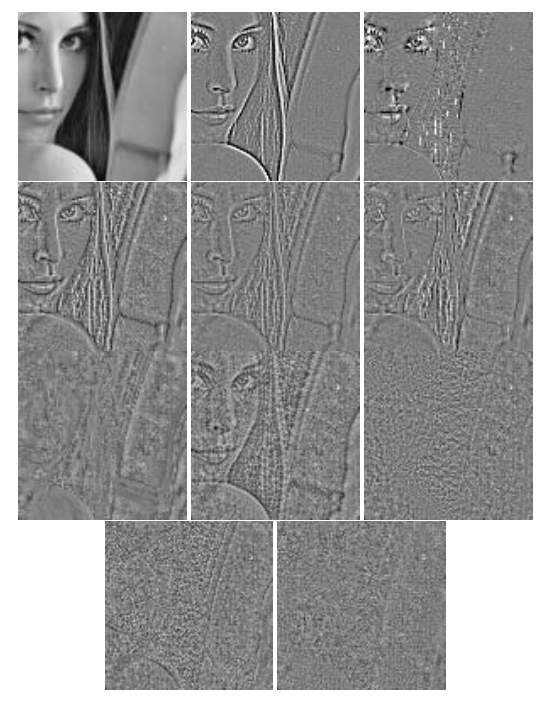
\includegraphics[scale=0.4]{method_noise}
\end{center}
 From left to right and from top to bottom:  original image,Gaussian convolution, mean curvature motion, total variation, Tadmor–Nezzar–Vese iterated total variation, Osher et al. total variation, neighborhood filter, soft TIWT, hard TIWT, DCT empirical Wiener filter, and the NL-means algorithm.\\
 \\
 You can see that the NL means algorithm is closest to white noise, as it is very difficult to make out the original image from the method noise, and so is the best in this area

\subsection{Mean square error}
\cite{machine_2018}The mean square error measures the average squared difference between the estimated values and what is estimated. In images this acts as a measure of how far from the true image the denoised image is. These results are taken from \cite{buades_review_2005}
\begin{center}
	\includegraphics[scale=0.7]{"mean"}
\end{center}
Here it can be seen that the NL-means algorithm gives images that are closest to the true image, and so performs best for image denoising under this measurement.
\newpage
\section{The influence of the algorithmic parameters on the output}
In the following images I am changing the values of h, the template window size and the search window size, from a standard set at h=5, template window size=7 and search window size =21. I will adjust each one in turn to show the differences yielded by changing them.

\begin{figure}[H]
	\centering
	\begin{subfigure}{.24\textwidth}
		\centering
		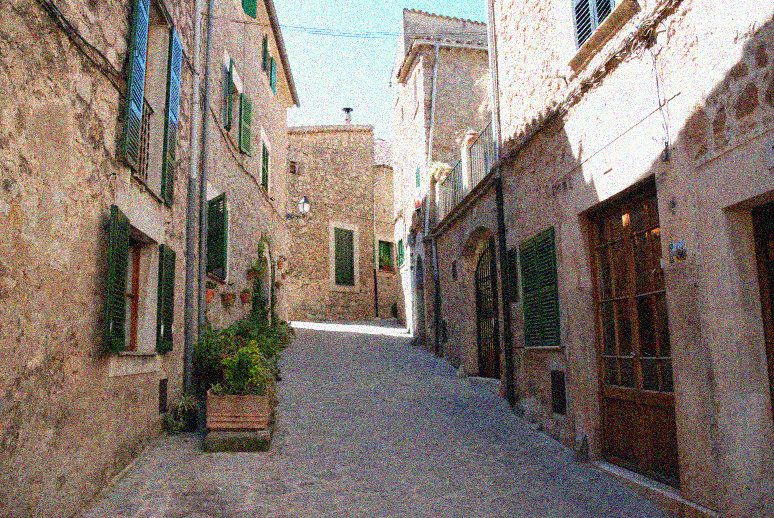
\includegraphics[width=\linewidth]{h2}
		\caption{h=2}
		\label{fig:h2}
	\end{subfigure}
	\begin{subfigure}{.24\textwidth}
		\centering
		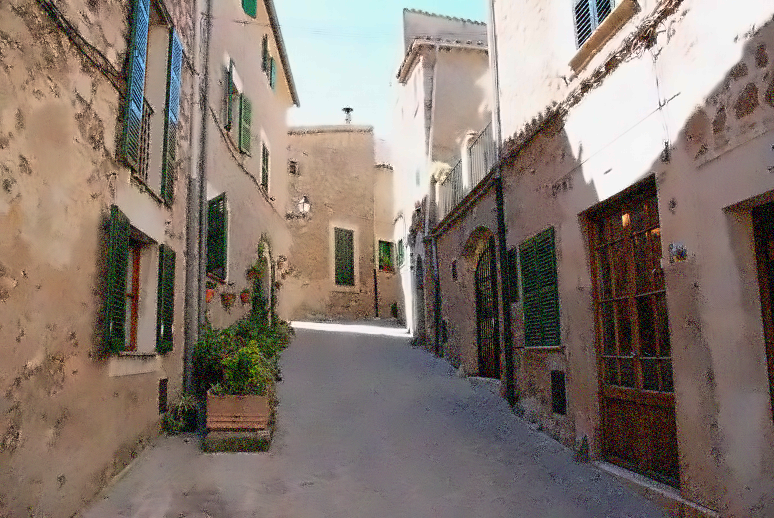
\includegraphics[width=\linewidth]{h10}
		\caption{h=10}
		\label{fig:h10}
	\end{subfigure}
	\begin{subfigure}{.24\textwidth}
		\centering
		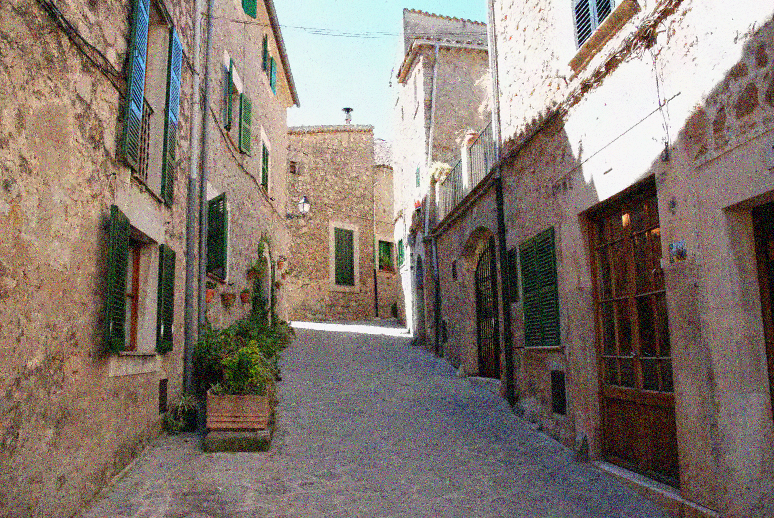
\includegraphics[width=\linewidth]{template2}
		\caption{template width=2}
		\label{fig:template2}
	\end{subfigure}
	\begin{subfigure}{.24\textwidth}
		\centering
		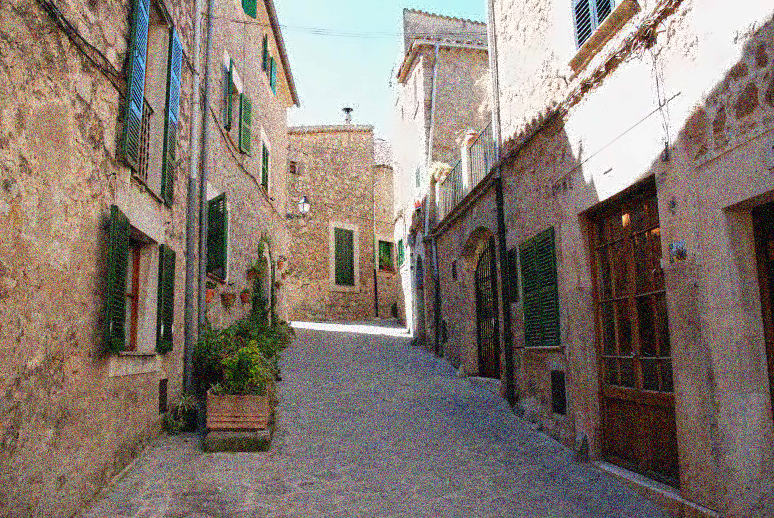
\includegraphics[width=\linewidth]{template15}
		\caption{template width=10}
		\label{fig:template15}
	\end{subfigure}
	\begin{subfigure}{.24\textwidth}
		\centering
		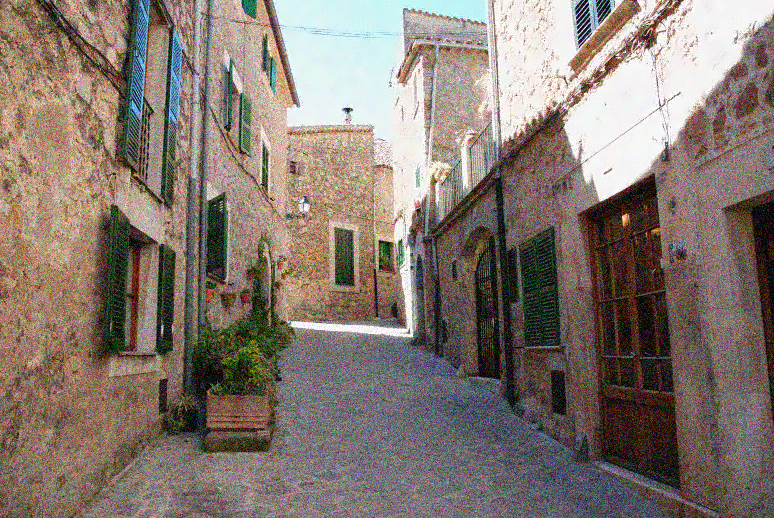
\includegraphics[width=\linewidth]{search10}
		\caption{search window size=10}
		\label{fig:search10}
	\end{subfigure}
	\begin{subfigure}{.24\textwidth}
		\centering
		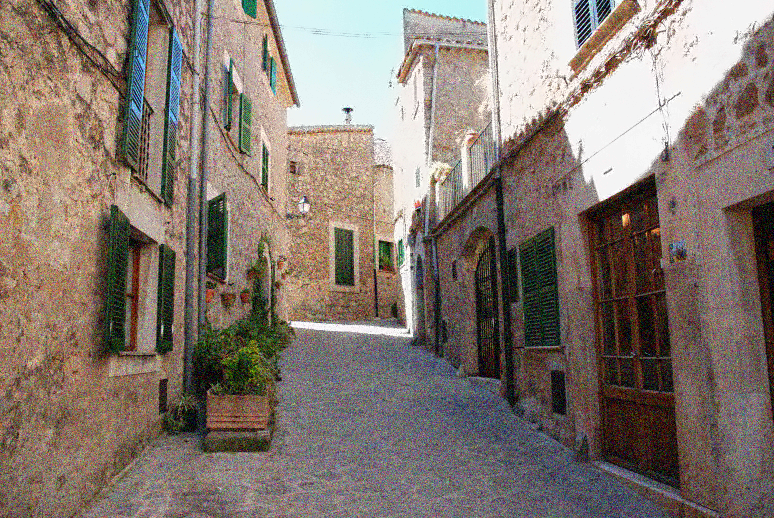
\includegraphics[width=\linewidth]{search30}
		\caption{search window size=30}
		\label{fig:search30}
	\end{subfigure}
	\caption{The effects of adjusting the value of the various parameters}
	\label{fig:parameters}
\end{figure}
By adjusting the value of h you get a large change in the amount of smoothing, although a large amount of noise is still present. Increasing the value of h does increase the PSNR from 28.60 to 29.66\\
\\
The effects from adjusting the template width are much more subtle than that of adjusting h, it can be noticed in the wires overhead that a larger template width has reduced the detail. An increase in the template width yields a small reduction in the PSNR from 28.68 to 28.51.\\
\\
The effects for the value of the search window are also very subtle, and again can only be noticed fully in the overhead wires. An increase in the search window yields a marginal increase in the PSNR from 28.51 to 28.52.


\section{Modifications and extensions of the algorithm that have been proposed in the literature}
\subsection{Testing stationarity}
\cite{buades_review_2005} One proposed modification is one to test stationarity. The original algorithm works under the conditional expectation process:
\begin{theorem}
(conditional expectation theorem)\\
Let $Z_j=\{X_j,Y_j\}$ for $j=1,2,...$ be a strictly stationary and mixing process. For $i\in I$, let $X$ and $Y$ be distributed as $X_i$ and $Y_i$. Let J be a compact subset $J\subset \mathbb{R}^p$ such that
$$\inf\{f_X(x);x\in J\}>0$$
\end{theorem}
However this is not true everywhere, as each image may contain exceptional, non-repeated structures, these would be blurred out by the algorithm, so the algorithm should have a detection phase and special treatment of nonstationary points. In order to use this strategy a good estimate of the mean and variance at every pixel is needed, fortunately the non-local means algorithm converges to the conditional mean, and the variance can just be calculated using $EX^2-(EX)^2$
\newpage
\subsection{Multiscale version}
Another improvement to make is one to speed up the algorithm, this is proposed using a multiscale algorithm.
\begin{enumerate}
	\item Zoom out the image $u_0$ by a factor of 2. This gives the new image $u_1$
	\item Apply the NL means algorithm to $u_1$, so that with each pixel of $u_1$, a list of windows centered in $(i_1,j_1)...(i_k,j_k)$ is associated
	\item For each pixel of $u_0$, $(2i+r,2j+s)$ with $r,s\in \{0,1\}$, we apply the NL means algorithm. However instead of comparing with all the windows in the search zone, we just compare with the 9 neighbouring windows of each pixel
	\item This procedure can be applied in a pyramid fashion
\end{enumerate}
\section{Applications of the original algorithm and its extensions}
\subsection{Medical Imaging}
\cite{zhang_applications_2017} It has been proposed that Non-Local means can be used in X-Ray imaging, allowing for a reduction of noise in the scans, making them easier to interpret. In CT scans a higher dose can be given to give a clearer image, but with that is more dangerous, however by applying the NL means algorithm a lower dose can be given for the same clarity. It benefits from the improvement stated above to test stationarity as the the noise and streak artifacts are non stationary. The original algorithm was also not good at removing the streak artifacts in low-flux CT images resulting from photon starvation. However by applying one-dimensional nonlinear diffusion in the stationary wavelet domain before applying the non-local means algorithm these could be reduced.
\subsection{Video Denoising}
\cite{ali_recursive_2017} NLM can also be applied in video denoising, it has an adaptation as the denoising can be improved by using the data from sequential frames. In the implementation proposed in the paper, the current input frame and prior output frame are used to form the current output frame. In the paper the measurements they make fail to show that this algorithm is an improvement from current algorithms, however the algorithm does have much better subjective visual performance.

\bibliographystyle{unsrtnat}
\bibliography{bibliography}
\newpage
\begin{appendices}
Image \ref{fig:h2}\\
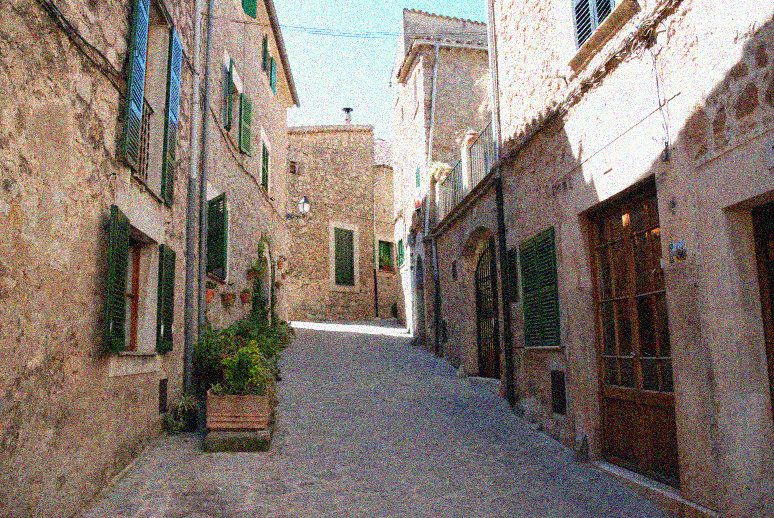
\includegraphics[width=0.8\linewidth]{h2}\\
Image \ref{fig:h10}\\
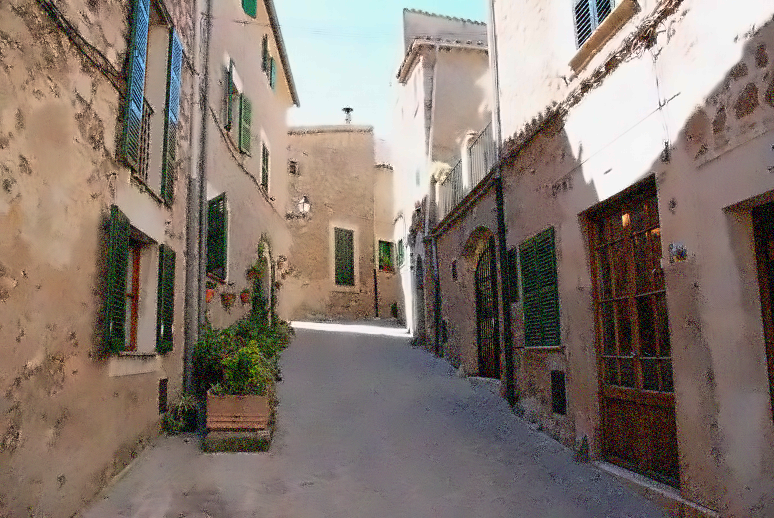
\includegraphics[width=0.8\linewidth]{h10}
\newpage
Image \ref{fig:template2}\\
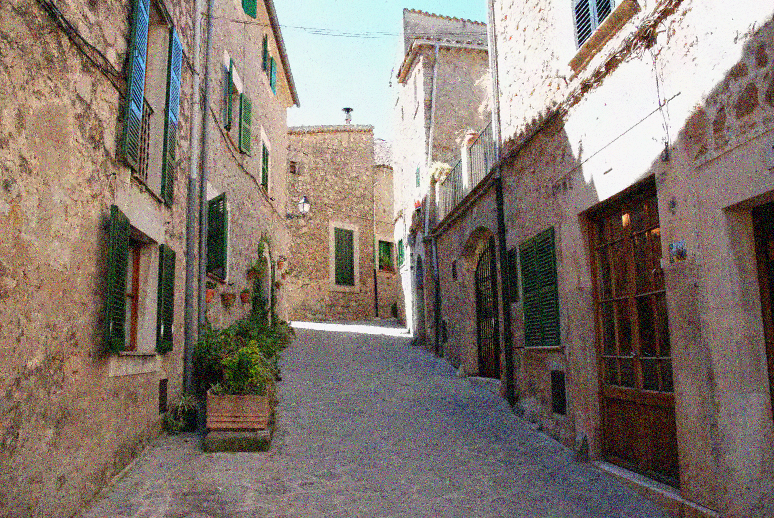
\includegraphics[width=0.8\linewidth]{template2}\\
Image \ref{fig:template15}\\
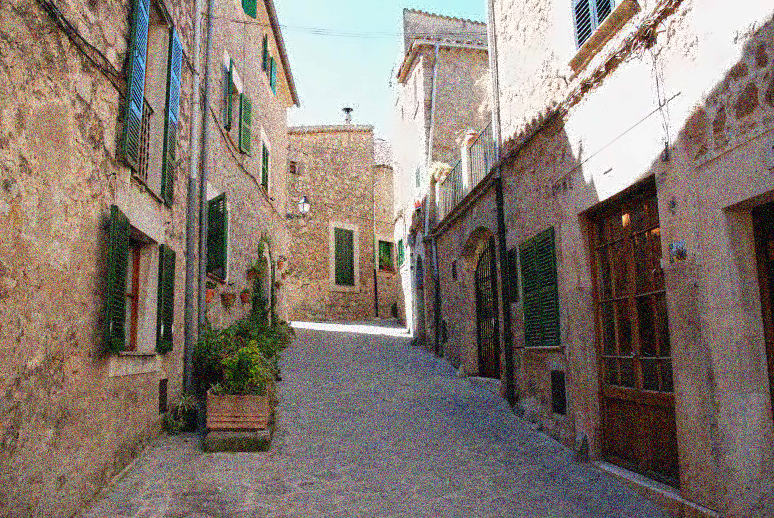
\includegraphics[width=0.8\linewidth]{template15}
\newpage
Image \ref{fig:search10}\\
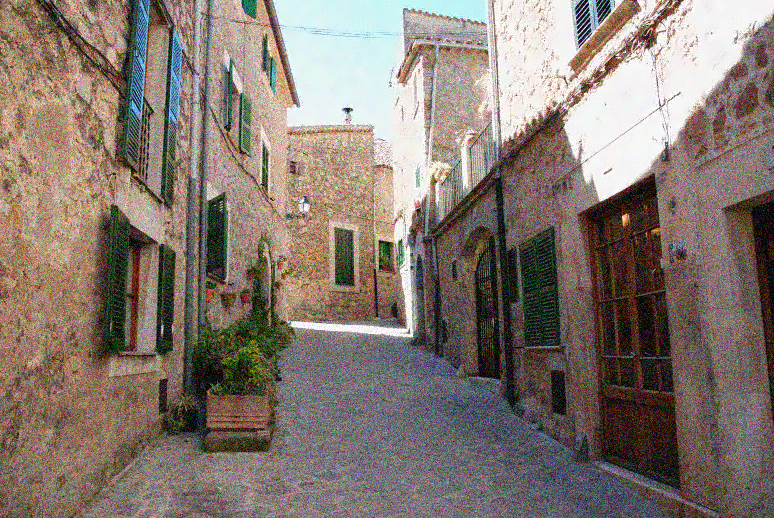
\includegraphics[width=0.8\linewidth]{search10}\\
Image \ref{fig:search30}\\
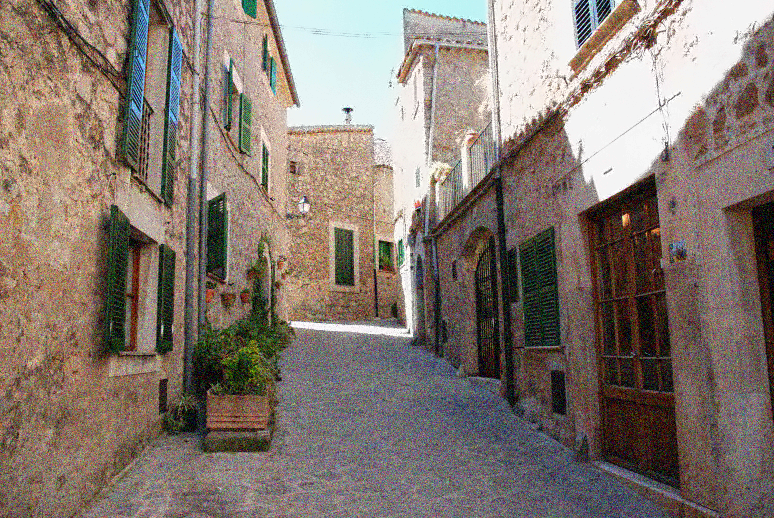
\includegraphics[width=0.8\linewidth]{search30}\\
\end{appendices}



\end{document}